\section{Precision Replacement Redistributes Success and Failure}
\label{sec:value}
\label{sec:r1}
\label{sec:r2}

\paragraph{Many rescues, many damages, small net.} Replacing an action with BF16's is a sensitive intervention of small net value. On the \tautwo{} development panel (85 tasks $\times$ 20 complete blocks), replacing a W4 agent's first tool-structure-divergent action with B's changes the task outcome in $M=15.5$--$20.9$\% of units (Figure~\ref{fig:case}b). Rescues and damages are of similar size, $r=6.8$--$11.4$ and $d=7.5$--$10.1$\pp{}, so the net gain $\Gall$ lies between $-1.9$ and $+2.9$\pp{}. Two fixed-pool intervals exclude zero (negative for q4 GPTQ-W4, positive for q8 GPTQ-W4); no new-task interval does. Pooled over the four W4 cells, $\Gall=+0.7$ [$-0.3$, $+1.6$]\pp{} with $M=18.6$\%. KV8 cells turn over fewer outcomes ($M=6.5$--$8.1$\%, a descriptive comparison). % src: analysis/fork/out/dev_all_20261001T070326Z.md
$\Gall$ is a local replacement effect, not an end-to-end comparison (Appendix~\ref{app:e2e}).

\paragraph{The same swap under two continuations.} The net effect hides how the action's value depends on what follows. On divergent states, the action swap's average effect is the same under Q's and under B's continuation (W4 pool: $\DQ=G=+0.5$ [$-0.7$, $+1.7$], $\DB=+0.5$ [$-1.0$, $+2.1$]\pp{}), and upgrading this step, the rest, or both has no detectable average gain ($H=+0.2$, $F=+0.7$\pp{}, all intervals covering zero). % src: analysis/fork/out/ghf_20261001T211519Z.md (§1 pools, W4:all; F - H = Δ_B)
State by state, however, the two effects often differ. In 26.9\% [25.7, 28.1] of pooled W4 divergent states (22.9--30.5\% per W4 cell; new-task interval 22.1--32.0\%), the swap has an effect under one continuation and a different one under the other; in the KV8 pool the share is 15.3\% [13.2, 17.3]. % src: analysis/fork/out/ghf_20261001T211519Z.md (§2; crossed column)
Strict reversals are rare (3.2\% of pooled W4 states); most off-diagonal states are an effect under one continuation and none under the other, as in Figure~\ref{fig:case}a. States where the swap helps more under Q ($I>0$, 13.6\%) and under B ($I<0$, 13.4\%) are about equally frequent, so the mean interaction is $+0.0$ [$-1.9$, $+2.0$]\pp{} although a quarter of states depend on the continuation. % src: analysis/fork/out/ghf_20261001T211519Z.md (TL;DR; §2, pool W4:all)
\begin{figure}[t]
\centering
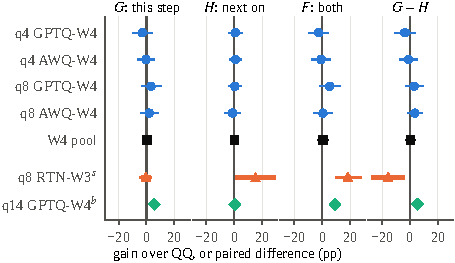
\includegraphics[width=\columnwidth]{figures/f9_upgrade_modes.pdf}
\caption{Value of the three upgrade modes on the same divergent states: replace this step ($G$), take over from the next step ($H$), or both ($F$); gain in success over QQ, pp. \tautwo{} development cells and pool: thick fixed-pool 95\%, thin new-task 95\%. $^s$Stress cell, three blocks ($t$ interval over block means). $^b$BFCL multi-turn, one run per item (item bootstrap 95\%). Within a row the three modes are paired; across rows, descriptive. All cells: Appendix Figure~\ref{fig:ghf} and Table~\ref{tab:ghf}.} % src: analysis/fork/out/ghf_20261001T211519Z.json; analysis/fork/out/ext_q14_20261002T085647Z.json
\label{fig:modes}
\end{figure}

\paragraph{Which upgrade mode pays depends on the configuration.} The 26.9\% is one description of this coupling; the design's use is that all three upgrade modes are measured on the same states (Figure~\ref{fig:modes}). In q8 GPTQ-W4 on the fixed task pool, replacing the action is worth $G=+3.3$ [$+1.6$, $+5.0$]\pp{}, taking over the continuation $H=+0.4$, and both $F=+5.4$; in q4 GPTQ-W4, B's action lowers success ($G=-2.9$ [$-5.7$, $-0.2$], unadjusted). These orderings are not confirmed on new-task intervals (Appendix~\ref{app:r2main}). % src: analysis/fork/out/ghf_20261001T211519Z.md (§1)
In the stress cell q8 RTN-W3 (three blocks), whose own success is low, the value lies in the continuation: $H=+15.3$ [$+0.7$, $+29.9$] and $F=+18.4$\pp{}, against $G=-0.4$ for the action alone. % src: analysis/fork/out/ghf_20261001T211519Z.md (§1)
For Qwen3-14B GPTQ-W4 on BFCL (one configuration, one run per item, 471 divergent items), it lies in the action: $G=+5.7$ [$+2.9$, $+8.7$], $H=+0.4$ [$-1.1$, $+1.9$], $F=+9.1$ [$+5.8$, $+12.5$]\pp{}, with only 6.4\% of states continuation-dependent. % src: analysis/fork/out/ext_q14_20261002T085647Z.md (§2; TL;DR)
A single upgrade mode chosen from averages or from one configuration would misprice the others.

\paragraph{Other states, tasks and environments.} The pattern is not specific to \tautwo{}'s simulated user or to development tasks. On BFCL multi-turn and ALFWorld, which have no simulated user (one run per item), the replacement turns over 5.2--24.6\% of items in both directions, and the off-diagonal share is 4.7--17.1\% in BFCL W4 cells and 32.8--40.0\% in q8 ALFWorld W4 cells (post hoc). % src: analysis/fork/out/ext_20261001T135106Z.md; analysis/fork/out/ext_r2_20261002T024433Z.md (§3, §6)
On 34 unseen telecom tasks, under a protocol frozen before any holdout unit ran (12 fresh blocks, three W4 cells, primary endpoint $\Gall$ on a crossed 90\% interval against $\pm$3\pp{}), the replacement again rescued and damaged ($r=+5.21$ [$+3.30$, $+7.11$], $d=+9.77$ [$+6.45$, $+13.10$]\pp{}) and task fragility repeated across independent nonce halves ($\rho=0.59$, $p=.0001$). The primary estimate was $\Gall=-4.57$\pp{} (crossed 90\% [$-7.17$, $-1.96$]). The pre-registered readings had no negative category, so the decisional reading is \emph{inconclusive}; outside them, the interval lies below zero. % src: analysis/fork/out/holdout_confirm_20261002T012353Z.md; docs/insights/PREREG_FORK_CONFIRM.md §0
At ordinary (Bank U) states, turnover is lower (W4 cells, U1 and U2B: 4.7--9.0\%), the net gain covers zero, and most outcome changes come from differences in text; their labels did not reproduce under a second user simulator, so we do not report them as a property of the action (Appendix~\ref{app:banku}). % src: analysis/fork/out/bank_u_f01_f02_f03_20261002T003037Z.md (§2); analysis/fork/out/simctrl_20261001T212742Z.md
